\documentclass[a4paper,11pt]{article}
\usepackage[T2A, T1]{fontenc}
\usepackage[utf8]{inputenc}
\usepackage[main=bulgarian, english]{babel}
\usepackage{indentfirst}
\usepackage{graphbox}
\usepackage{amsmath}
\usepackage{multirow}
\usepackage{booktabs}
\usepackage{xcolor}
\usepackage{listings}
\lstset{basicstyle=\ttfamily,
  showstringspaces=false,
  commentstyle=\color{red},
  keywordstyle=\color{blue}
  escapeinside={\%*}{*)},
}
\lstdefinestyle{tree}{
    texcl=true,
    literate=
    {├}{{\smash{\raisebox{-1ex}{\rule{1pt}{\baselineskip}}}\raisebox{0.5ex}{\rule{1ex}{1pt}}}}1 
    {│}{{\smash{\raisebox{-1ex}{\rule{1pt}{\baselineskip}}}\raisebox{0.5ex}{\rule{1ex}{0pt}}}}1
    {─}{{\raisebox{0.5ex}{\rule{1.5ex}{1pt}}}}1 
    {└}{{\smash{\raisebox{0.5ex}{\rule{1pt}{\dimexpr\baselineskip-1.5ex}}}\raisebox{0.5ex}{\rule{1ex}{1pt}}}}1 
}

\usepackage{float}
\usepackage{multirow}
\usepackage{tabularx}
\usepackage{hyperref}
\usepackage{graphicx} % Include figure files
\usepackage{dcolumn} % Align table columns on decimal point
\usepackage{bm} % bold math
\usepackage{subcaption}
% \usepackage[style=mla, backend=biber, dashed=false]{biblatex}
\usepackage[super, square]{natbib}
% \setcounter{biburllcpenalty}{7000}
% \setcounter{biburlucpenalty}{8000}
% \usepackage{bibentry}
% \nobibliography{references}

% FILL OUT THE DETAILS BELOW:
\newcommand{\firstauthor}{Даниел Халачев}
\newcommand{\secondauthor}{Цветелина Чакърова}
\newcommand{\thirdauthor}{Николета Бейска}
\title{NoProp}
% \date{An optional custom date, the default is today}
\newcommand{\subtitle}{Трениране на невронни мрежи без back-propagation или forward-propagation}
\newcommand{\firststudentnumber}{4MI3400603}
\newcommand{\secondstudentnumber}{8MI3400591}
\newcommand{\thirdstudentnumber}{2MI3400639}
\newcommand{\program}{Извличане на информация и откриване на знания}
\newcommand{\course}{Дълбоко обучение с Тензорфлоу, летен семестър 2024/2025}
\newcommand{\firstsupervisor}{проф. Милен Чечев}
\newcommand{\secondsupervisor}{Александър Захарян}
\newcommand{\thirdsupervisor}{Алексис Датсерис}
\renewcommand{\lstlistingname}{Програмен код}

\usepackage[onehalfspacing]{setspace} % Increase line spacing
\usepackage[margin=2.5cm]{geometry} % Modify margins
\usepackage{graphicx,booktabs} % Packages for images, tables, and APA citations

\usepackage[dvipsnames]{xcolor}
\hypersetup{
    colorlinks=true,
    linkcolor=black,
    citecolor=CadetBlue,
    filecolor=CadetBlue,      
    urlcolor=CadetBlue,
}

\begin{document}
\begin{titlepage}
\makeatletter
\begin{center}
	\textsc{Софийски университет "Св. Климент Охридски"}
	\par \textsc{Факултет по математика и информатика}
	\par Специалност "\program"
    \par Курс "\course"

	\vfill \hrule height .08em \bigskip
	\par\huge\@title\bigskip
	\par\Large\subtitle\bigskip
	\hrule height .08em\normalsize
	
	\vfill
	
\includegraphics[width=\textwidth,height=0.25\textheight,keepaspectratio]{images/SU.png} % The EUR logo, but this could also be another image
	\vfill
	
	\begin{tabular}{lll}
    \toprule
    \multirow{3}{*}{Изготвили:} & \firstauthor, & ФН: \firststudentnumber; \\
                                & \secondauthor, & ФН: \secondstudentnumber; \\
                                & \thirdauthor, & ФН: \thirdstudentnumber;\\
    \midrule
    \multirow{3}{*}{Ръководители:} & \multicolumn{2}{l}{\firstsupervisor;} \\
                                    & \multicolumn{2}{l}{\secondsupervisor;} \\
                                    & \multicolumn{2}{l}{\thirdsupervisor} \\
    \midrule
    Дата: & \multicolumn{2}{l}{\@date} \\
    \bottomrule
\end{tabular}

	
	\vfill
\end{center}
\makeatother
\end{titlepage}
\newpage

\newpage

\tableofcontents
\newpage


\section{Въведение}

\subsection{Мотивация}

Тренирането на невронни мрежи чрез методите \textbf{back-propagation} и \textbf{forward-propagation} е в основата на съвременните подходи за машинно самообучение. Тези методи, макар и доказали своята ефективност, имат \textbf{ограничения}. Сред тях са: необходимост от последователно изпълнение на двата етапа; високи изисквания за памет за изчисляване на градиентите; трудности при паралелизация; загуба на контекст. Тези недостатъци мотивират изследователите да търсят алтернативни подходи за обучение, които да са по-ефективни, гъвкави и мащабируеми.

\subsection{Подобрение на сегашните методи}

В статията \emph{NoProp: Training Neural Networks without Back-propagation or Forward-propagation}\cite{li2025noproptrainingneuralnetworks} е предложен новаторски подход за обучение на невронни мрежи, който избягва използването на посочените традиционни методи. Той е вдъхновен е от дифузионните модели, които се обучават да премахват различни нива на шум. По подобен начин \emph{NoProp} премахва различни нива на шум, но всеки слой се обучава независимо без \emph{forward-propagation} и \emph{back-propagation} през целия модел. Твърди се, че това позволява паралелна обработка, намалява изискванията за памет и ускорява обучението, като същевременно запазва или подобрява точността на класификация в сравнение с други методи без \emph{back-propagation}. \emph{NoProp} има три варианта - \emph{NoProp-DT} (дискретно време), \emph{NoProp-CT} (непрекъснато време) и \emph{NoProp-FM} (flow matching).

\subsection{Цел}
Статията описва впечатляващи резултати от проведените експерименти, но е публикувана без официален програмен код. В допълнение, измерванията са извършени единствено върху набори от данни с ниска резолюция (\texttt{MNIST}, \texttt{CIFAR-10}, \texttt{CIFAR-100}). Възникват въпроси относно стабилността на модела при по-сложни задачи. 
Целта на този проект е да се изследва и приложи подходът \emph{NoProp}, за да се провери неговата ефективност и потенциал за подобрения. Проектът имплементира вариантите \emph{NoProp-DT} и  \emph{NoProp-СТ}, тества ги върху посочените набори от данни, както и върху база данни с изображения с по-висока резолюция - \texttt{BLOODMNIST}.

\subsection{Мотивация за избора на NoProp-DT и NoProp-CT}

Проектът се фокусира върху два от трите възможни разновидности на модела, а именно на \emph{NoProp-DT} и \emph{NoProp-CT}. Този избор се основава на резултатите, докладвани в оригиналната статия, където тези два варианта демонстрират по-висока точност и стабилност в сравнение с \emph{NoProp-FM}.

\newpage

\section{Кратко въведение в NoProp архитектурата}

В тази секция се коментират само най-важните моменти от оригиналната \emph{NoProp} статия\cite{li2025noproptrainingneuralnetworks}, тъй като основен фокус на текущата документация е да представи разработената имплементация и експериментите, проведени над нея.

\subsection{Архитектура на NoProp}
\subsubsection{Фаза на извод}
По време на извод входните данни се обработват в серия от стъпки, като всяка стъпка представлява трансформаця на данните, чрез прекарването им през \textbf{дифузионен блок}. Мрежата получава като вход началното изображение \(x\), което е обект на класификация, и Гаусов шум \(z_{0}\). На всяка стъпка се създава нова латентна променлива \(z_t\). Всеки блок \(u_{t}\) е зависим от променливата от предишната стъпка \(z_{t-1}\) и входното изображение за цялата мрежа \(x\). 

След $t$ на брой преобразувания получаваме редицата от променливи $z_{1}, z_{2}, \dots, z_{t}$. Последната от тях се подава на линеен слой и \emph{softmax} активираща функция, които позволяват използването на научените характеристики с цел класификация. 

\begin{figure}[H]
    \centering
    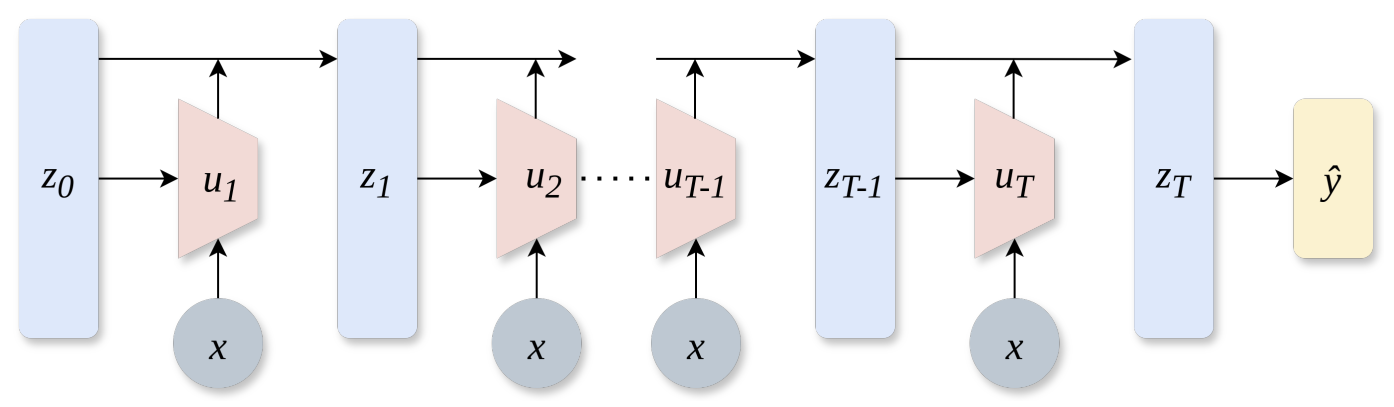
\includegraphics[width=6.26in,keepaspectratio]{images/NoProp Inference Architecture.png}
    \caption{Архитектура на фазата на извод. $z_1, z_2, \dots, z_t$ са последователните етапи на трансформация на първоначалния шум $z_0$. $u_1, u_2, \dots u_T$ са дифузионните блокове, които се обучават да премахват различни нива на шум. Линейният слой и \emph{softmax} активиращата функция не са изобразени експлицитно.}
    \label{no_prop_arch}
\end{figure}
По време на извод тензорите се подават на слоевете последователно през цялата мрежа, както в традиционна невронна мрежа. Но на фигура \ref{no_prop_arch} се забелязва първата съществена разлика с повечето \emph{backpropagation} алгоритми - входното изображение $x$ се подава на всеки блок $u_t$, а не еднократно на входа на модела. 

\subsubsection{Фаза на обучение}
Фазата на обучение е ключова за подхода \emph{NoProp}, тъй като всеки дифузионен блок \(u_t\) се разглежда като самостоятелна невронна мрежа, която се обучава независимо от останалите. Това позволява по-лесна паралелизация на обучението и намалява изискванията за памет. Линейният слой, използван за класификация, се тренира едновременно с всички блокове, за да се осигури съгласуваност на научените характеристики и предотвратява срив в ембедингите на класовете.

\subsection{Структура на дифузионния блок}
Дифузионният блок в двата варианта \emph{NoProp-CT} и \emph{NoProp-DT} има общи структурни сегменти:
\begin{itemize}
    \item\textbf {кодиране на изображението}
    \begin{itemize}
        \item\textbf{конволюционни слоеве} - извличат характеристики от входното изобраение чрез прилагане на конволюционни филтри върху него. Сегментът наподобява \emph{ResNet} конволюционна мрежа
        \item \textbf{напълно свързан слой} - свежда извлечените характеристики до ембединги с консистентен размер
    \end{itemize}
    \item\textbf{кодиране на предходния етикет} - силно варира в двата варианта, но включва напълно свързани слоеве и \emph{ReLU} активации
    \item\textbf{конкатениращ сегмент} - обединява ембедингите на различните кодирания.
\end{itemize}

В допълнение, блокът на \emph{NoProp-CT} включва и сегмент за \textbf{кодиране на времевите последователности}. 

\subsection{NoProp-DT}
Изображението се обработва в краен брой стъпки $T$, които са параметър на модела.  

\begin{figure}[H]
    \centering
    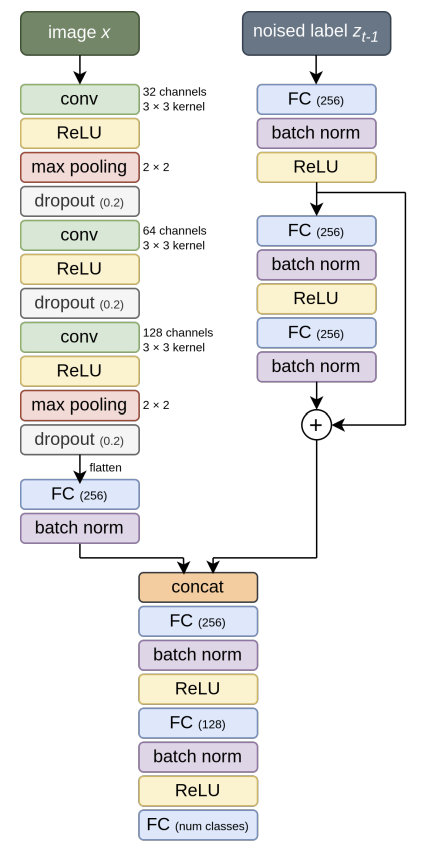
\includegraphics[width=3.00in,keepaspectratio]{images/NoProp-DT Model.png}
    \caption{Модел фазата на трениране на NoProp-DT}
\end{figure}

Кодирането на изображението \(x\) се осъществява чрез конволюционни слоеве \emph{conv} (32, 64, 128 канала; ядра 3x3), слоеве с активационни функции \emph{ReLU}, max pooling 2x2, \emph{dropout} с вероятност 0.2 и \emph{flatten}, последван от напълно свързан \emph{FC} слой и нормализация. Латентната променлива \(z_{t-1}\) се обработва чрез FC слоеве и batch нормализация, както и \(ReLu\) активация, на два етапа, които се свързват чрез \emph{skip connection}. 
Кодиранията се конкатенират и прекарват през напълно-свързани слоеве, batch нормализация и \(ReLU\) двукратно. 
Дифузионният блок завършва с напълно свързан слой с размерност броя възможни класове, за да се извърши класификация.

\subsection{NoProp-CT}
Архитектурата на NoProp-CT във фазата на трениране е идентична с тази на NoProp-DT със следната разлика: на входа, освен изображението \(x\), се подава и времеви параметър \(t\), който кодира времевата зависимост чрез \emph{positional embeddings}. Съответно всеки блок \(u_{t}\) приема и времевия параметър \(t\). Всяка поетапна трансформация се адаптира според етапа на дифузия, като по този начин моделът може да "знае" колко е напреднал процесът.
\begin{figure}[H]
    \centering
    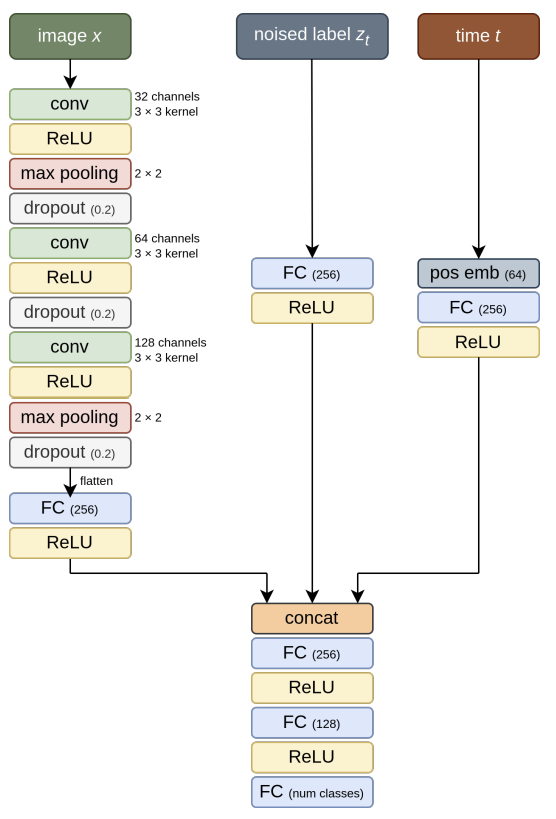
\includegraphics[width=3.00in,keepaspectratio]{images/NoProp-CT Model.png}
    \caption{Модел фазата на трениране на NoProp-CT}
\end{figure}


Кодирането на изображението \(x\) почти аналогично с \emph{NoProp-DT} варианта. Разликата е в последния слой преди конкатенацията - в NoProp-DT има batch нормализация, а тук - \(ReLU\). Латентната променлива \(z_t\) се обработва чрез FC слой и \(ReLU\). В допълнение се приема и променлива за времето \(t\), което липсва в \emph{NoProp-DT}. Тя преминава през слой за позиционно кодиране с 64 единици, FC слой и \(ReLU\). Трите кодирания се конкатенират и прекарват през напълно свърза слой и \(ReLU\) активация двукратно. Блокът отново завършва с напълно свързан слой с размерност броя класове при класификация.

\subsection{Псевдокод на тренирането}

В статията са представени циклите за обучение на разновидностите на модела чрез псевдокод, за да се илюстрира по-ясно процеса на оптимизация на модела. Обучителният набор от данни стандартно се разделя на части (\emph{batches}) и цикълът се изпълнява за всеки бач. Изчислената загуба за всеки бач оптимизира параметрите на модела. 

\textbf{Вход:}
\begin{itemize}
    \item \(T\) - Брой на дискретните стъпки в процеса на дифузия 
    \item \(\{(x_{i}, y_{i})_{i=1}^{n}\}\) - Набор от данни, състоящ се от двойки входни данни и етикети $(x_{i}, y_{i})$
    \item \(B\) - batch size
    \item \(\eta\) - Константа, която контролира мащаба на регуляризацията - прави едната част от цялата загубата да има по-голямо значение.
    \item \(W_{Embed}\) - Матрица с кодирания на класовете, която преобразува етикетите \(y_{i}\) във векторни представяния \(u_{y_{i}}\)
    \item \(\{\theta_{t}\}_{t=1}^{T}\) или $\theta$, \(\theta_{out}\) - Параметри на модела
    \item \(\{\alpha_{t}\}_{t=1}^{T}\) или \(\bar{\alpha_{t}}\) - Noise scheduler. Последователност, която определя нивото на шум, добавено към данните в зависимост от времето
\end{itemize}

\subsubsection{NoProp-DT}

\begin{figure}[H]
    \centering
    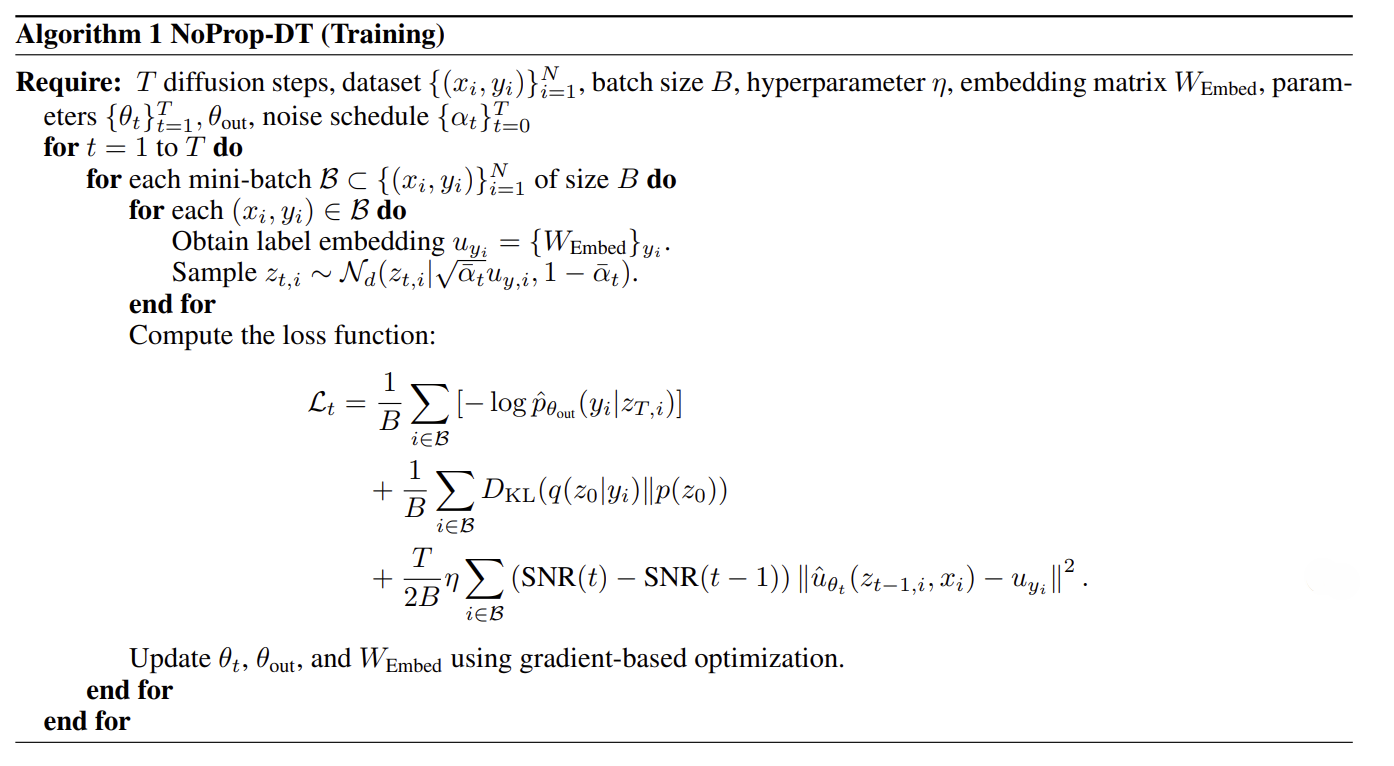
\includegraphics[width=6.26in,keepaspectratio]{images/NoProp-DT Training Pseudocode.png}
    \caption{Псевдокод за фазата на трениране на NoProp-DT}
\end{figure}

\textbf{Основни стъпки:}
За всяка стъпка времева \(t\) обхождаме всеки mini-batch \(\mathcal{B}\) от входните данни с размер \(B\). За всяка двойка \((x_{y}, y_{i})\) от \(\mathcal{B}\) извличаме векторното представяне \(u_{y_{i}}\) на етикета и генерираме шум \(z_{t, i}\) с нормално разпределение. След това изчисляваме функцията на загуба за \(\mathcal{B}\). Обновяваме параметрите \(theta_{t}\), \(theta_{out}\) и \(W_{Embed}\) чрез градиентно-базирана оптимизация. \\

\textbf{Функция на загуба:}
Функцията на загуба е съставена от три събираеми, които имат следните роли:
\begin{itemize}
    \item $\mathbf{\frac{1}{B} \sum\limits_{i\in\mathcal{B}}{\left[ -\log \hat{p}_{\theta_{\text{out}}}(y_i | z_{T,i}) \right]}}$ - загуба от тип отрицателна логаритмична вероятност (negative log-likelihood loss). Измерва колко добре моделът може да възстанови оригиналните данни от шумния сигнал \(z_{T,i}\). Загубата намалява, когато моделът предсказва правилния етикет \(y_{i}\) с по-висока вероятност.
    \item $\mathbf{\frac{1}{B}\sum\limits_{i \in \mathcal{B}} D_{\text{KL}}(q(z_0|y_i) \| p(z_0))}$ - загуба от тип KL дивергенция (Kullback-Leibler divergence). Измерва разликата между наученото разпределение и желаното априорно разпределение. Регуларизира латентното пространство, като го принуждава да следва определено разпределение. Загубата намалява, когато латентното пространство \(q(z_0|y_i)\) се приближава до априорното разпределение \(p(z_0\).
    \item $\mathbf{\frac{T}{2B} \eta \sum\limits_{i \in \mathcal{B}} (\text{SNR}(t) - \text{SNR}(t-1)) \left\| \hat{u_{\theta_t}}(z_{t-1,i}, x_i) - u_{y_i} \right\|^2}$ - загуба от тип квадратична разлика (Mean Squared Error) с тегло, базирано на Signal-to-Noise Ratio. Насочва обучението да адаптира параметрите така, че да възстановяват оригиналните представяния на етикетите от шумните данни. Теглото \((\text{SNR}(t) - \text{SNR}(t-1))\) дава по-голямо значение на определени времеви стъпки. \(\eta\) контролира относителната важност на това събираемо. Загубата намалява, когато моделът точно предсказва шума \(u_{y_{i}}\).
\end{itemize}

\subsubsection{NoProp-CT}

\begin{figure}[H]
    \centering
    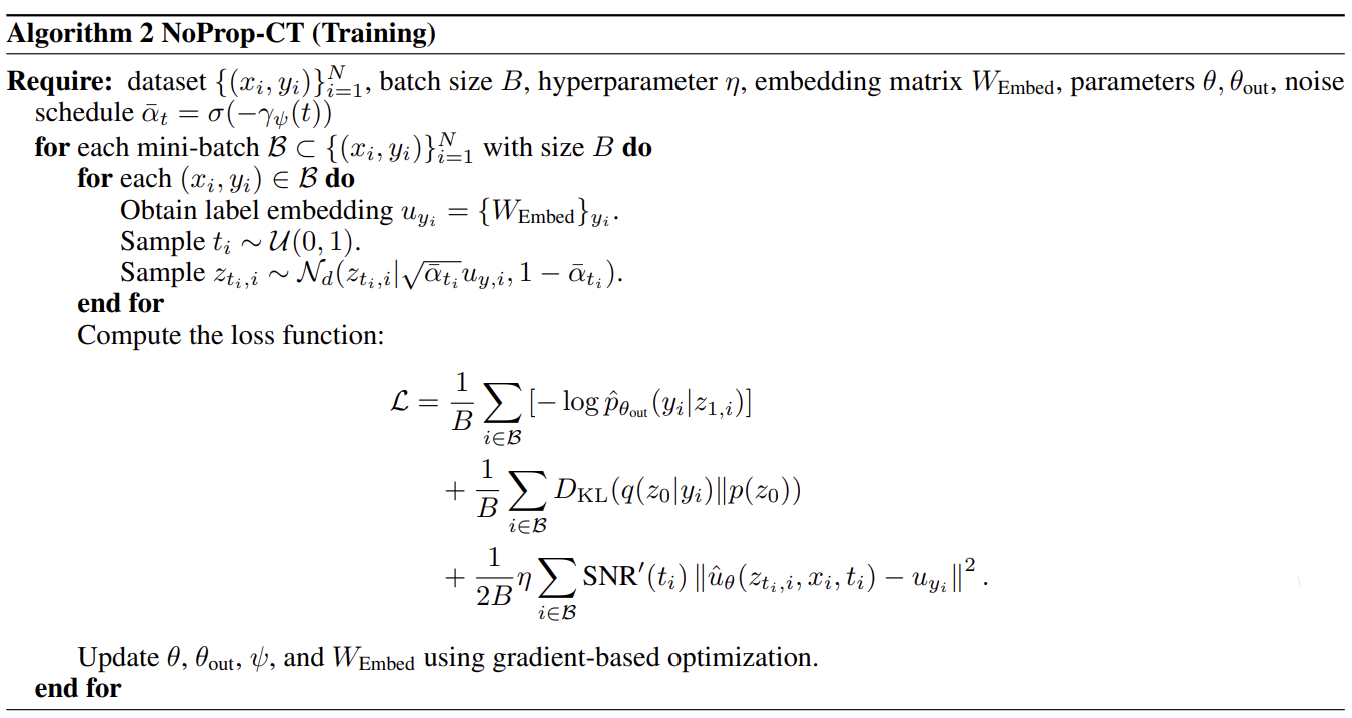
\includegraphics[width=6.26in,keepaspectratio]{images/NoProp-CT Training Pseudocode.png}
    \caption{Псевдокод за фазата на трениране на NoProp-CT}
\end{figure}

\textbf{Основни стъпки:}
Обхождаме всеки mini-batch \(\mathcal{B}\) от входните данни с размер \(B\). За всяка двойка \((x_{y}, y_{i})\) от \(\mathcal{B}\) извличаме векторното представяне \(u_{y_{i}}\) на етикета, избираме случайно време \(t_{i}\) чрез непрекъснато равномерно разпределение \(U(0, 1)\) и генерираме шум \(z_{t, i}\) с нормално разпределение. След това изчисляваме функцията на загубата за \(\mathcal{B}\). Обновяваме параметрите \(\theta\), \(\theta_{out}\) и \(W_{Embed}\) чрез градиентно-базирана оптимизация. \\

\textbf{Функция на загуба:}
Функцията на загуба е съставена от три събираеми, които имат следните роли:
\begin{itemize}
    \item \(\mathbf{\frac{1}{B} \sum\limits_{i \in \mathcal{B}} \left[ -\log \hat{p}_{\theta_{\text{out}}}(y_i | z_{1,i}) \right]}\) - със същата роля като в \emph{NoProp-DT}.
    \item \(\mathbf{\frac{1}{B} \sum\limits_{i \in \mathcal{B}} D_{\text{KL}}(q(z_0|y_i) \| p(z_0))}\) - със същата роля като в \emph{NoProp-DT}.
    \item \(\mathbf{\frac{1}{2B} \eta \sum\limits_{i \in \mathcal{B}} \text{SNR}'(t_i) \left\| \hat{u}_\theta(z_{t_i,i}, x_i, t_i) - u_{y_i} \right\|^2}\) - загуба от тип квадратична разлика (Mean Squared Error) с тегло, базирано на Signal-to-Noise Ratio. Със същата роля като в \emph{NoProp-DT}. Различава се по липсата на константата $Т$. \(\text{SNR}'(t_i)\) е производната на Signal-to-Noise Ratio, която дава различни тегла на различните времеви моменти \(\eta\) контролира относителната важност на това събираемо. Загубата намалява, когато моделът точно предсказва шума \(u_{y_{i}}\).
\end{itemize}

\subsection{Препратки към оригиналната статия}

Следните части от оригиналната статия са ключови за по-детайлно запознаване с идеите  \emph{NoProp}:

\begin{itemize}
    \item Техническо описание на \emph{NoProp} (Раздел 2, страници 2–5) - 
Подробно описание на алгоритъма, включително математическата му основа.
    \item Експериментални резултати (Раздел 4, страници 6–9)
\end{itemize}

\section{Реализация}
\subsection{Структура}
Алгоритъмът е имплементиран на \lstinline{Python} с помощта на библиотеката \lstinline{PyTorch}. Реализацията е базирана на псевдокода, включен в научната работа \textit{NoProp: Training Neural Networks without Back-propagation or Forward-propagation}.\cite{li2025noproptrainingneuralnetworks}
\subsection{GitHub}
Целият програмен код може да бъде намерен на адрес \url{https://github.com/DanielHalachev/NoProp}.
\newpage

\begin{lstlisting}[style=tree, language=bash]
NoProp
├── config_data # Папка с конфигурационни файлове за всяка двойка набор и алгоритъм
└── src         
    ├── components  
    │   ├── backbone.py # Eкстрактор на характеристики в диф. блок
    │   ├── block.py # Абстрактен клас за диф. блокове
    │   ├── concatenator.py # Абстрактен клас, комбинира кодиранията
    │   ├── ct_block.py # Имплементация на диф. блок за NoProp-CT
    │   ├── ct_concatenator.py # Комбинира изходи за CT версията 
    │   ├── ct_noise_scheduler.py # Управлява шумa за CT версията
    │   ├── dt_block.py # Имплементация на диф. блок за NoProp-DT
    │   ├── dt_concatenator.py # Комбинира изходи за DT версията 
    │   ├── dt_noise_scheduler.py # Управлява шума за DT версията 
    │   ├── noise_scheduler.py # Абстрактен клас за управление на шума
    │   ├── resnet_type.py # Дефинира видовете ResNet архитектури
    │   └── time_scheduler.py # Генератор на времеви последователности
    ├── data  
    │   ├── cifar100_dataset.py # Зарежда и подготвя данните от CIFAR-100 
    │   ├── dataset_manager.py # Менажира всички възможни набори от данни 
    │   ├── medmnist_dataset.py # Зарежда и подготвя данните от MedMNIST+ 
    │   └── mnist_dataset.py # Зарежда и подготвя данните от MNIST  
    ├── embedings  
    │   ├── ct_label_encoder.py # Енкодер на етикети за NoProp-CT
    │   ├── dt_label_encoder.py # Енкодер на етикети за NoProp-DT
    │   ├── label_encoder.py # Абстрактен базов клас за енкодерите на етикети
    │   ├── sinusoidal_embedding.py  # Изчислява синусоидални ембединги
    │   └── time_encoder.py # Енкодер на времето
    ├── models  
    │   ├── base_model.py # Абстрактен базов клас за всички NoProp модели
    │   ├── model_type.py # Дефинира идентификатори за моделите CT, DT и FM
    │   ├── model_wrapper.py # Обвивка около NoProp моделите с тр. метаданни
    │   ├── noprop_ct.py # Имплементация на BaseNoPropModel за CT
    │   └── noprop_dt.py # Имплементация на BaseNoPropModel за DT
    ├── scripts  
    │   └─── train_test.py # Обучава и тества модела с помощта на train\_utils
    └─── utils  
        ├── device.py # Клас, който определя най-подходящото устройство за обучение
        ├── model_config.py # Дефинира класове за конфигурация на \emph{NoProp} модел
        ├── test_utils.py # Тества NoProp модел върху тестово множество от данни
        ├── train_config.py # Управлява параметрите за обучение на NoProp
        └── train_utils.py # Полезни функции за обучението
\end{lstlisting} 
\subsection{Особености}
\paragraph{Инициализиране с прототипи}
Ембедингите на класовете (матрицата $W_\text{Embed}$ се инициализират с прототипи, което е един от вариантите, описани в статията. 

\paragraph{Алгоритми за извод}
Тъй като \emph{NoProp} е вдъхновен от дифузионните модели, екипът имплементира алтернативни алгоритми за извод по методите на Ойлер и Хюн. Използването им не доведе до повишаване на резултатите. 

\paragraph{Изчисляване на Cross-Entropy Loss}
В процеса на обучение на модела, екипът установи, че използването на изхода от напълно свързаните слоеве и \emph{softmax}, както е описано в статията, е полезно за \emph{NoProp-CT}, но значително влошава стабилността на трениране при \emph{NoProp-DT}. Екипът постигна поведението на \emph{NoProp-DT}, описано в статията, чрез директно използване на логитите, изведени от дифузионните блокове. 

\paragraph{Набор с висока резолюция}
За да тества възможностите на модела, екипът извърши експеримент с тренировъчния набор \texttt{MedMNIST+}, който поддържа резолюция 128x128 пиксела. 

\paragraph{Optimizer}
Екипът експериментира с \emph{Adam} и \emph{AdamW} при по-слабо представящите се комбинации набор-вариант на \emph{NoProp}, но не установи подобрение. Затова изследването се придържаше към оптимизаторите, описани в статията. 

\paragraph{Scheduler}
Екипът експериментира с добавянето на scheduler с 5000 \emph{warmup} стъпки, но това доведе до изненадващо влошаване на стабилността на обучението и много ниски резултати на тренировъчното множество върху всички набори от данни. 

\subsection{Хиперпараметри}
Хиперпараметрите на модела са зададени в конфигурационните файлове спрямо статията. Те могат да бъдат обобщени в следната таблица:

\begin{table}[H]
  \centering
  % \renewcommand{\arraystretch}{1.5} 
  \begin{tabular}{m{0.4\linewidth} m{0.6\linewidth}}
    \toprule
    \textbf{Параметър} & \textbf{Описание} \\
    \midrule
    \texttt{batch\_size} & Определя броя на обучителните примери, обработвани заедно в една итерация на обучението, което влияе на ефективността и стабилността му. \\
    \midrule
    \texttt{epochs} & Броят на епохите. Епоха представлява един пълен цикъл на обучението през целия набор от данни. \\
    \midrule
    \texttt{optimiser} & Оптимизатор на обучението, регулиращ градиентното спускане, адаптирайки скоростта на обучение спрямо временното представяне. \\
    \midrule
    \texttt{learning\_rate} & Размерът на стъпката при актуализирането на параметрите на модела и влияе върху скоростта и стабилността на сходимостта. \\
    \midrule
    \texttt{weight\_decay} & Този параметър добавя регуляризация към загубата, предотвратявайки прекомерна сложност в модела чрез намаляване на теглата. \\
    \midrule
    \texttt{number\_of\_timesteps} & Броя на времевите стъпки в NoProp-DT \\
    \midrule
    \texttt{eta} & Коефициент за регулиране значимостта на третия член на загубата. \\
    \midrule
    \texttt{embedding\_dimension} & Размерност на ембедингите $z_t$. \\
    \midrule
    \texttt{label\_encoder\_hidden\_dimension} & Размерността на ембедингите в скритите слоеве на енкодера на етикетите. \\
    \midrule
    \texttt{time\_encoder\_hidden\_dimension} & Размерността на ембедингите в скритите слоеве на енкодера на времето. \\

    \bottomrule
  \end{tabular}  
  \caption{Описаниe на хиперпараметрите}
  \label{tab:hyperparameters}
\end{table}

\begin{table}[H]
  \centering
  \renewcommand{\arraystretch}{1.5} % Увеличаване на вертикалния интервал
  \begin{tabular}{lcccccccc}
    \toprule
    \textbf{Набор} & \textbf{Вариант} & \textbf{Бач} & \textbf{Епохи} & \textbf{Опт.} & \textbf{lr} & \textbf{wd} & \textbf{Стъпки} & \textbf{$\eta$} \\
    \midrule
    MNIST & NoProp-DT & 128 & 100 & AdamW & 0.001 & 0.001 & 10 & 0.1 \\
    CIFAR-10 & NoProp-DT & 128 & 150 & AdamW & 0.001 & 0.001 & 10 & 0.1 \\
    CIFAR-100 & NoProp-DT & 128 & 150 & AdamW & 0.001 & 0.001 & 10 & 0.1 \\
    BLOODMNIST & NoProp-DT & 128 & 100 & AdamW & 0.001 & 0.001 & 1000 & 0.1 \\
    MNIST & NoProp-CT & 128 & 100 & Adam & 0.001 & 0.001 & 1000 & 1 \\
    CIFAR-10 & NoProp-CT & 128 & 500 & Adam & 0.001 & 0.001 & 1000 & 1 \\
    CIFAR-100 & NoProp-CT & 128 & 1000 & Adam & 0.001 & 0.001 & 1000 & 1 \\
    BLOODMNIST & NoProp-CT & 128 & 1000 & Adam & 0.001 & 0.001 & 1000 & 1 \\
    \bottomrule
  \end{tabular}
  \caption{Стойности на хиперпараметри за различни множества от данни и алгоритми. \texttt{lr} обозначава \texttt{learning\_rate}, \texttt{wd} - \texttt{weight\_decay}, а стъпките се отнасят до фазата на извод. }
  \label{tab:hyperparameters_values}
\end{table}

\section{Експерименти}

Имплементираният съгласно статията модел премина обучение на следния хардуер:
\begin{lstlisting}
CPU: Intel Xeon E5-2690 v4
GPU: NVIDIA GeForce RTX 4070 Ti SUPER

CPU: AMD EPYC 7702 64-Core Processor
GPU: NVIDIA RTX 4090
\end{lstlisting}

Данните бяха съхранявани систематично с помощта на платформата \emph{Weights \& Biases}. 

Двата варианта на модела са тренирани над различни множества данни, като постигнатите резултати са представени на графиките по-долу. За данните, представени в оригиналната статия - \texttt{MNIST}, \texttt{CIFAR-10} и \texttt{CIFAR-100}, са използвани стойностите на хиперпараметрите посочени в нея (Таблица \ref{tab:hyperparameters_values}). Представените стойности на постигнатите резултати са от извадки от три отделни експеримента на обучение, данните за които могат да се видят на графиките. Изборът на извадки от три експеримента балансира статистическа значимост и хардуерните наличности на екипа. 

\subsection{NoProp-DT и MNIST}

\begin{figure}[H]
    \centering
    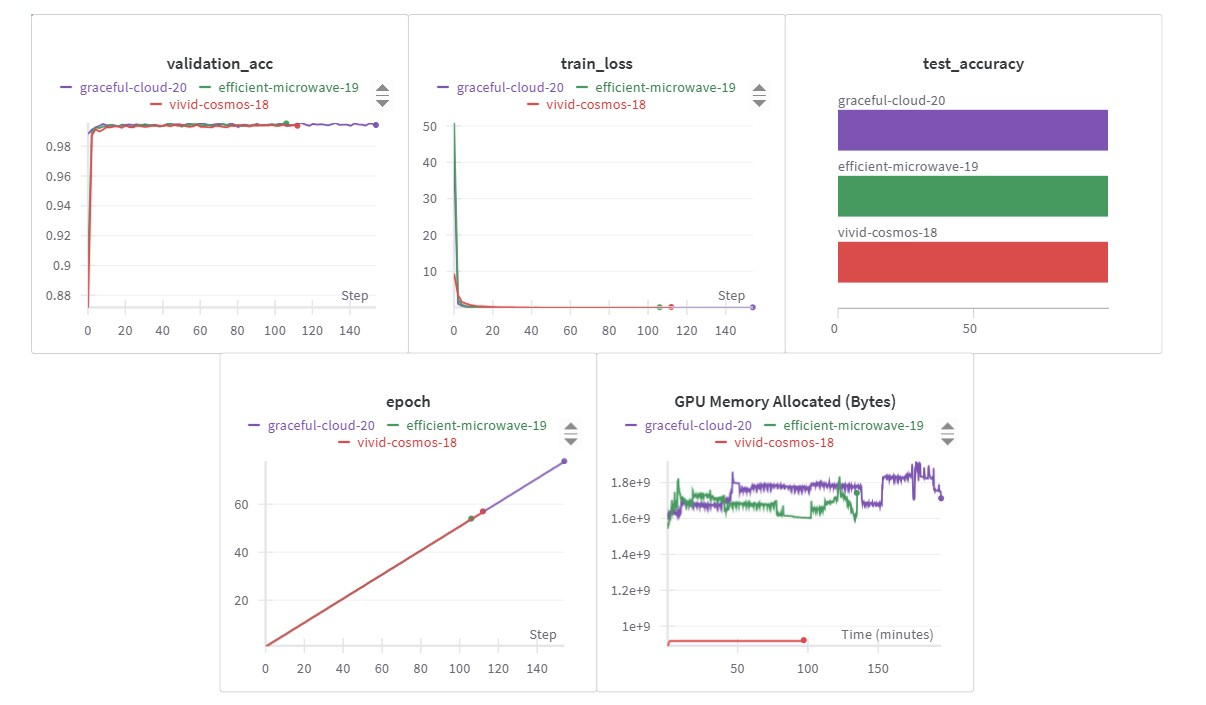
\includegraphics[width=6.26in,keepaspectratio]{images/NoProp-DT MNIST.jpg}
    \caption{Графични резултати за NoProp-DT върху MNIST}
\end{figure}

\begin{table}[H]
  \centering
  \renewcommand{\arraystretch}{1.5} % Увеличаване на вертикалния интервал
  \begin{tabular}{ccccc}
    \toprule
    \textbf{Име на изпълнение} & \textbf{Загуба} & \textbf{Тестова точност} & \textbf{Брой епохи} & \textbf{GPU памет (GB)}\\
    \midrule
    graceful-cloud-20 & 0.0875 & 99.42 & 78 & 1.92\\
    efficient-microwave-19 & 0.1151 & 99.53 & 54 & 1.84\\
    vivid-cosmos-18& 0.1743& 99.37& 57& 0.86\\

    \bottomrule
  \end{tabular}
  \caption{Метрики за различни изпълнения на NoProp-DT върху MNIST}
  \label{tab:avg_metrics_noprop_dt_mnist}
\end{table}

\subsection{NoProp-DT и CIFAR-10}

\begin{figure}[H]
    \centering
    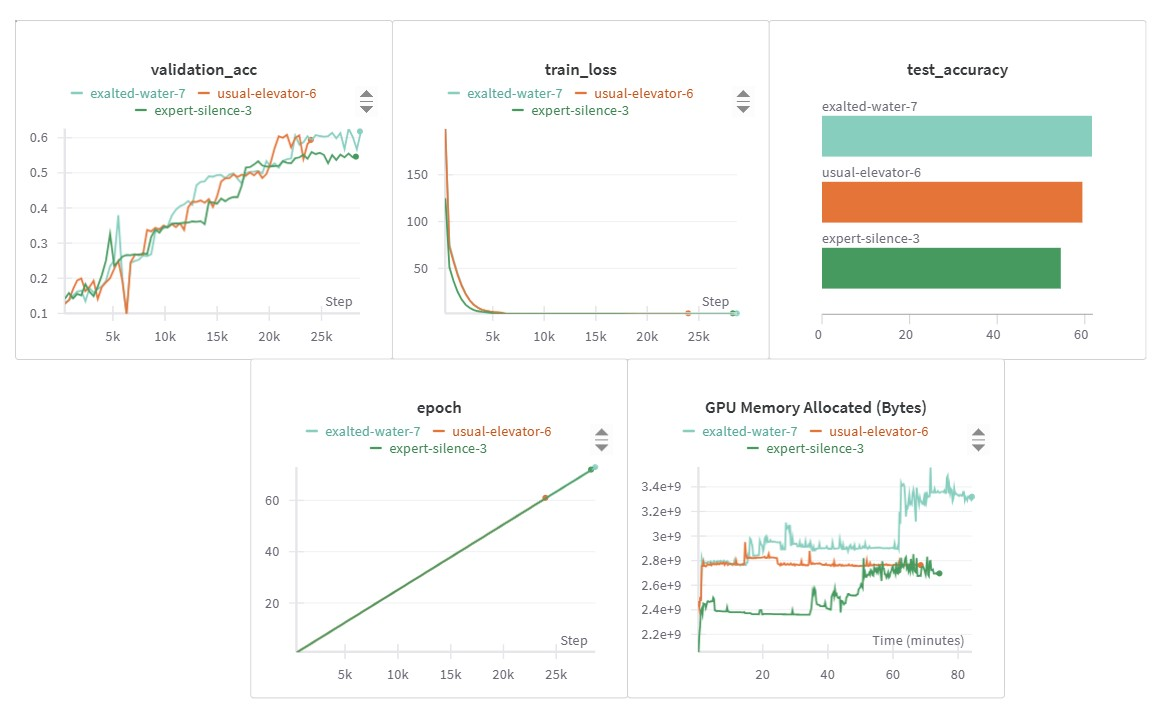
\includegraphics[width=6.26in,keepaspectratio]{images/NoProp-DT CIFAR10.jpg}
    \caption{Графични резултати за NoProp-DT върху CIFAR-10}
\end{figure}

\begin{table}[H]
  \centering
  \renewcommand{\arraystretch}{1.5} % Увеличаване на вертикалния интервал
  \begin{tabular}{ccccc}
    \toprule
    \textbf{Име на изпълнение} & \textbf{Загуба} & \textbf{Тестова точност} & \textbf{Брой епохи} & \textbf{GPU памет (GB)}\\
    \midrule
    helpful-gorge-6 & 1.3370 & 80.54 & 150 & 0.69\\
    curious-waterfall-5 & 1.4325 & 79.62 & 150 & 1.84\\
    fancy-terrain-1 & 1.2189 & 80.75 & 150 & 0.91\\
    \bottomrule
  \end{tabular}
  \caption{Метрики за различни изпълнения на NoProp-DT върху CIFAR-10}
  \label{tab:avg_metrics_noprop_dt_cifar-10}
\end{table}

\subsection{NoProp-DT и CIFAR-100}

\begin{figure}[H]
    \centering
    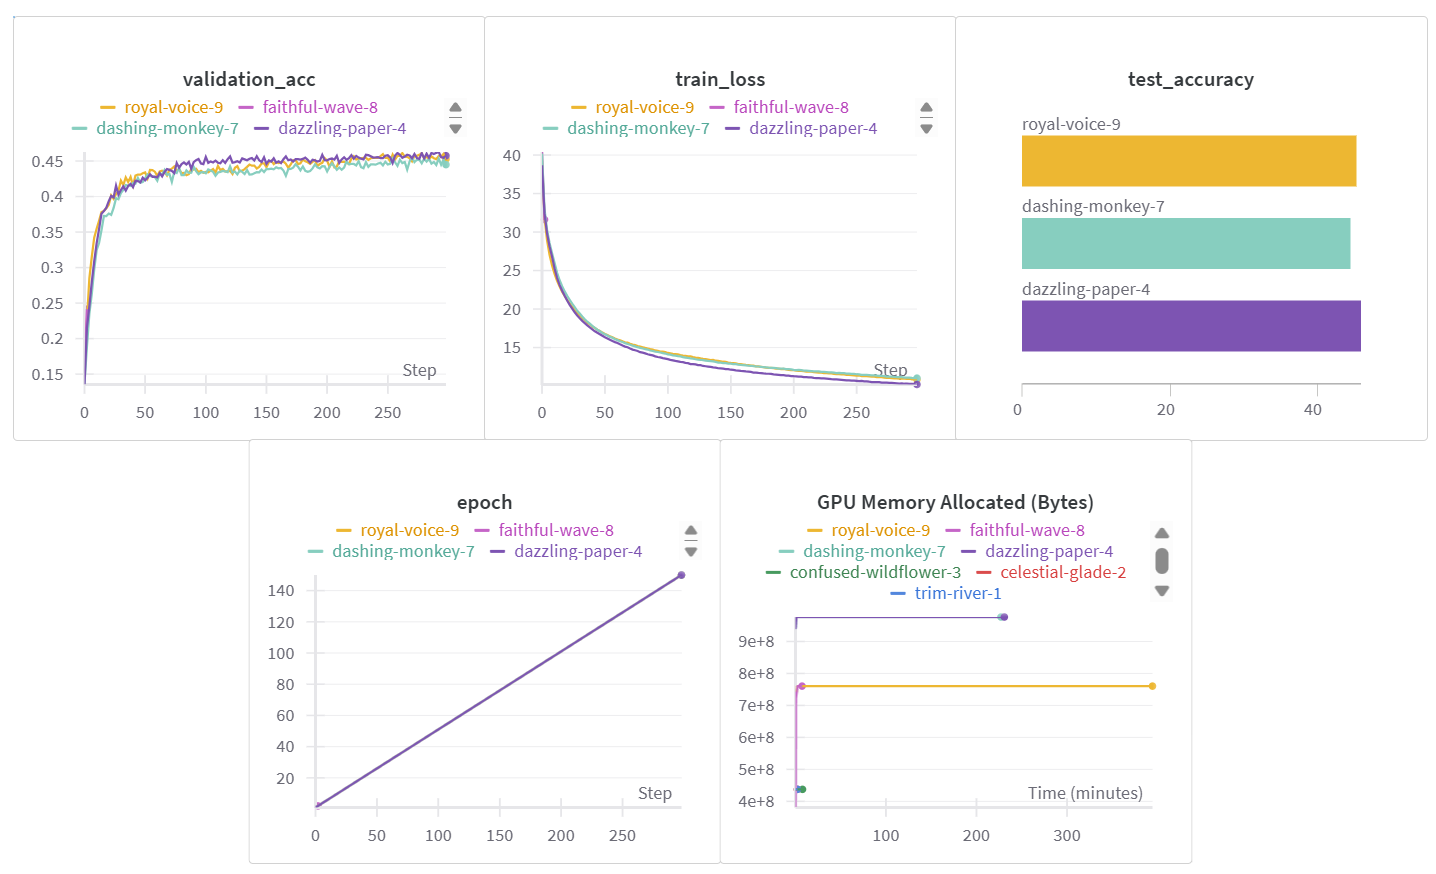
\includegraphics[width=6.26in,keepaspectratio]{images/NoProp-DT CIFAR-100.png}
    \caption{Графични резултати за NoProp-DT върху CIFAR-100}
\end{figure}

\begin{table}[H]
  \centering
  \renewcommand{\arraystretch}{1.5} % Увеличаване на вертикалния интервал
  \begin{tabular}{ccccc}
    \toprule
    \textbf{Име на изпълнение} & \textbf{Загуба} & \textbf{Тестова точност} & \textbf{Брой епохи} & \textbf{GPU памет (GB)}\\
    \midrule
    royal-voice-9& 10.8631& 45.27& 150 & 0.71\\
    dashing-monkey-7 & 11.0258 & 44.49 & 150 & 0.98\\
    dazzling-paper-4 & 10.2014 & 45.75 & 150 & 0.98\\
    \bottomrule
  \end{tabular}
  \caption{Метрики за различни изпълнения на NoProp-DT върху CIFAR-100}
  \label{tab:avg_metrics_noprop_dt_cifar-100}
\end{table}

\subsection{NoProp-DT и BLOODMNIST}

\begin{figure}[H]
    \centering
    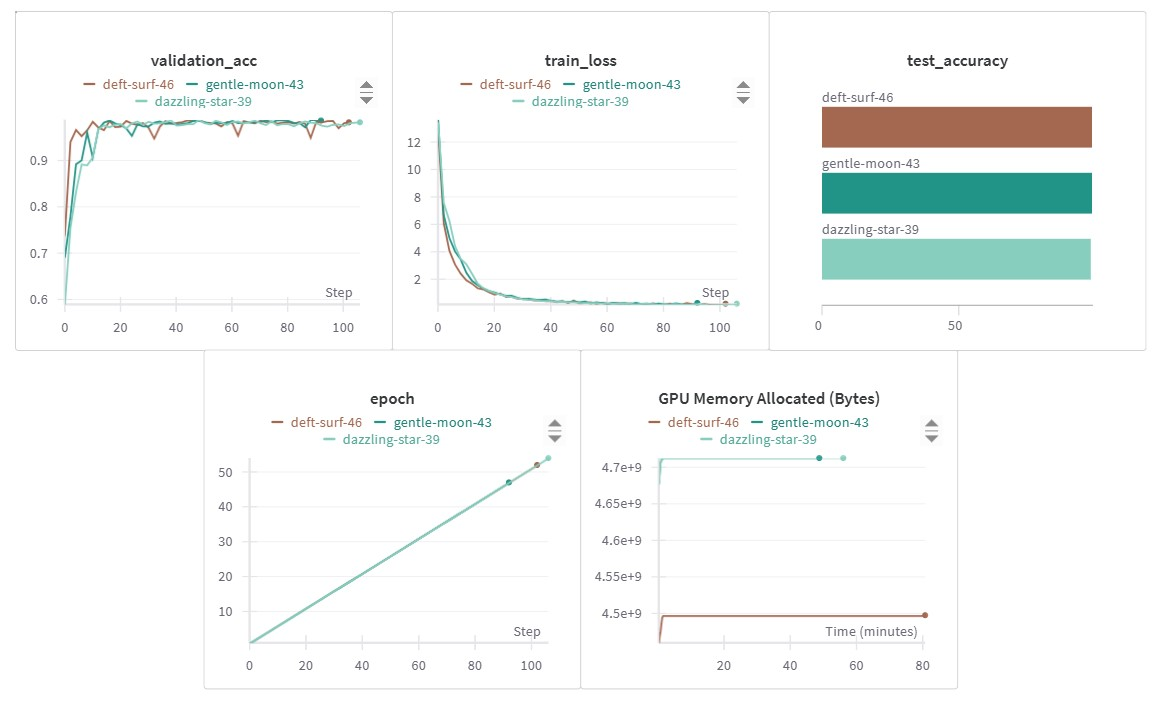
\includegraphics[width=6.26in,keepaspectratio]{images/NoProp-DT BLOODMNIST.jpg}
    \caption{Графични резултати за NoProp-DT върху BLOODMNIST}
\end{figure}

\begin{table}[H]
  \centering
  \renewcommand{\arraystretch}{1.5} % Увеличаване на вертикалния интервал
  \begin{tabular}{ccccc}
    \toprule
    \textbf{Име на изпълнение} & \textbf{Загуба} & \textbf{Тестова точност} & \textbf{Брой епохи} & \textbf{GPU памет (GB)}\\
    \midrule
    deft-surf-46 & 0.2152 & 98.25 & 52 & 4.50\\
    gentle-moon-43 & 0.2713 & 98.42 & 47 & 4.71\\
    dazzling-star-39 & 0.2163 & 97.98 & 54 & 4.71\\
    \bottomrule
  \end{tabular}
  \caption{Метрики за различни изпълнения на NoProp-DT върху BLOODMNIST}
  \label{tab:avg_metrics_noprop_dt_bloodmnist}
\end{table}

\subsection{NoProp-CT и MNIST}

\begin{figure}[H]
    \centering
    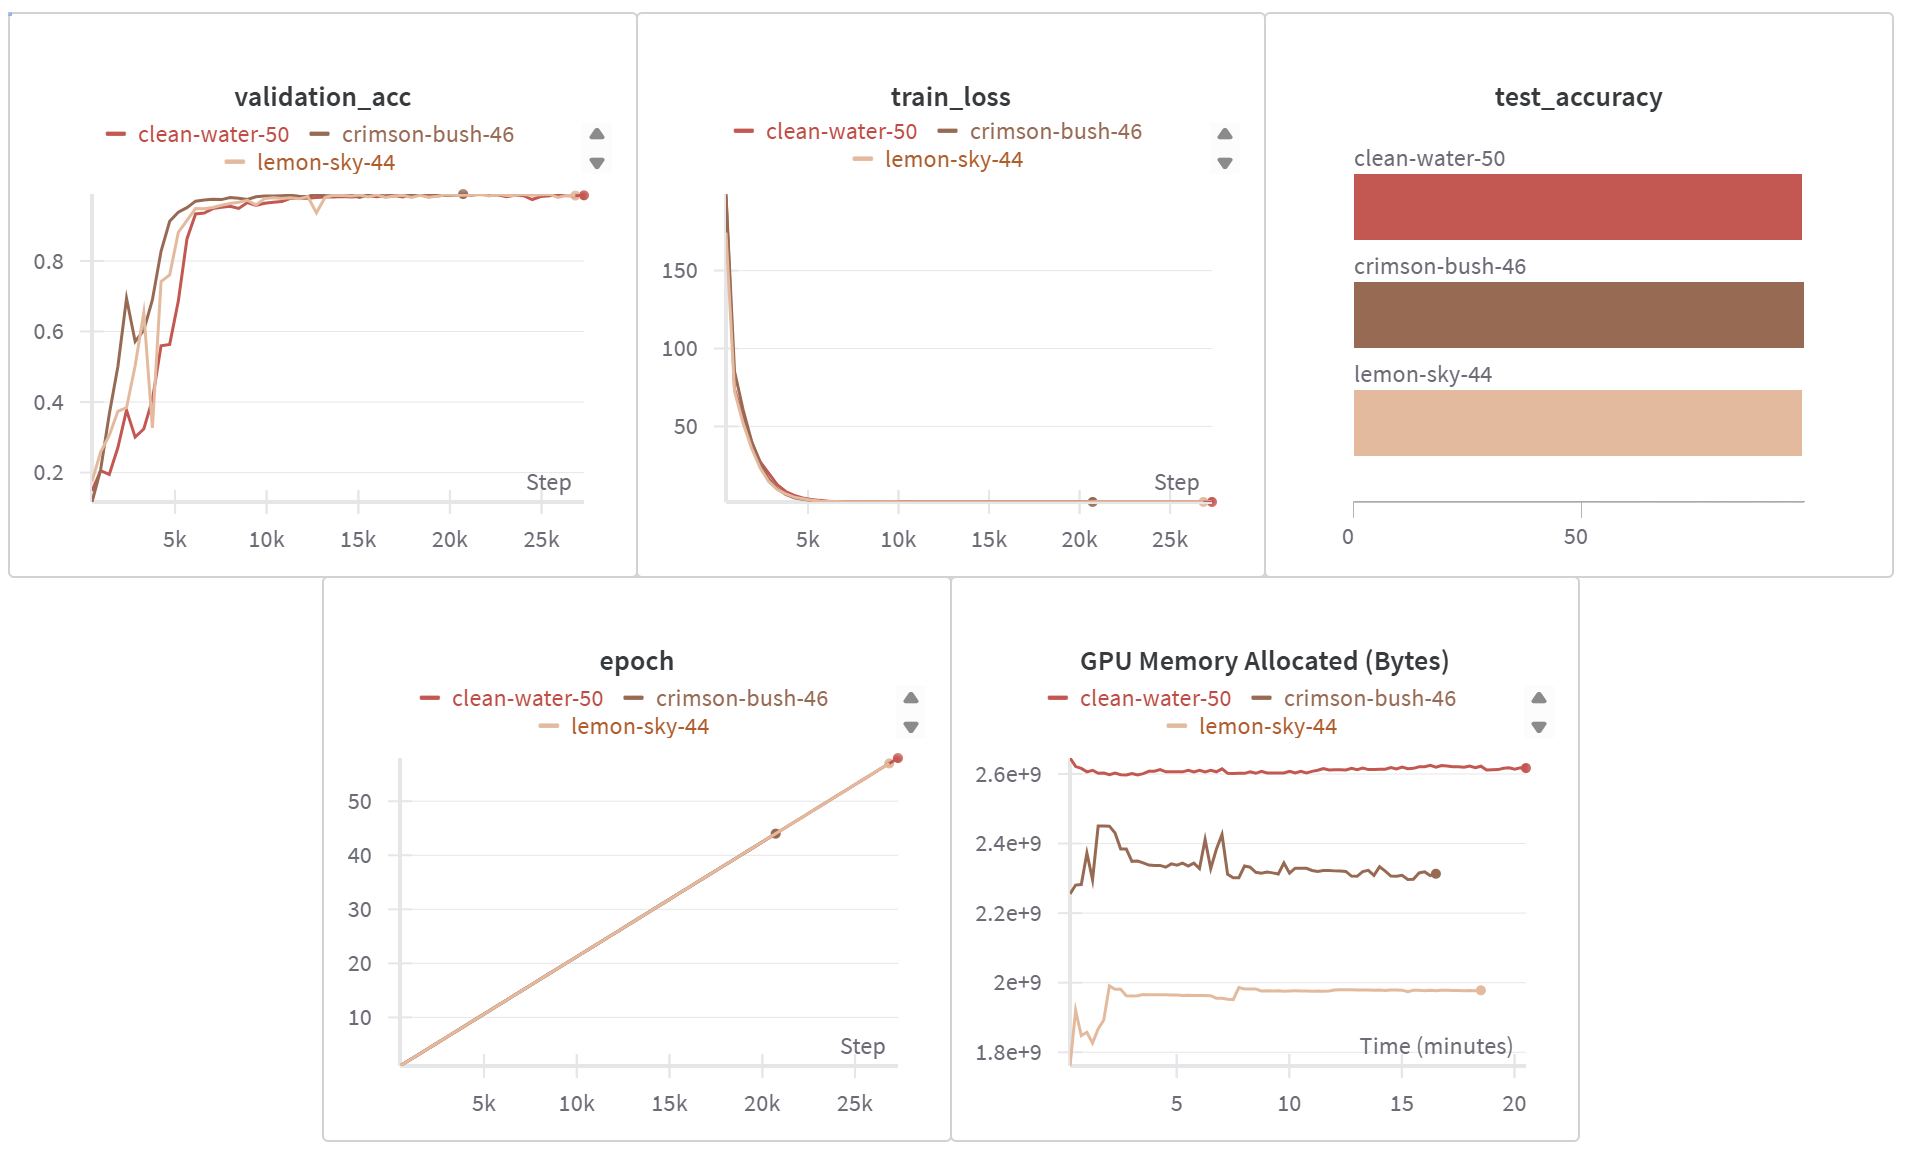
\includegraphics[width=6.26in,keepaspectratio]{images/NoProp-CT MNIST.png}
    \caption{Графични резултати за NoProp-CT върху MNIST}
\end{figure}

\begin{table}[H]
  \centering
  \renewcommand{\arraystretch}{1.5} % Увеличаване на вертикалния интервал
  \begin{tabular}{ccccc}
    \toprule
    \textbf{Име на изпълнение} & \textbf{Загуба} & \textbf{Тестова точност} & \textbf{Брой епохи} & \textbf{GPU памет (GB)}\\
    \midrule
    clean-water-50 & 1.4221 & 98.63 & 58 & 2.65\\
    crimson-bush-46 & 1.4950 & 99 & 44 & 2.45\\
    lemon-sky-44 & 1.4934 & 98.57 & 57 & 1.99\\
    \bottomrule
  \end{tabular}
  \caption{Метрики за различни изпълнения на NoProp-CT върху MNIST}
  \label{tab:avg_metrics_noprop_ct_mnist}
\end{table}


\subsection{NoProp-CT и CIFAR-10}

\begin{figure}[H]
    \centering
    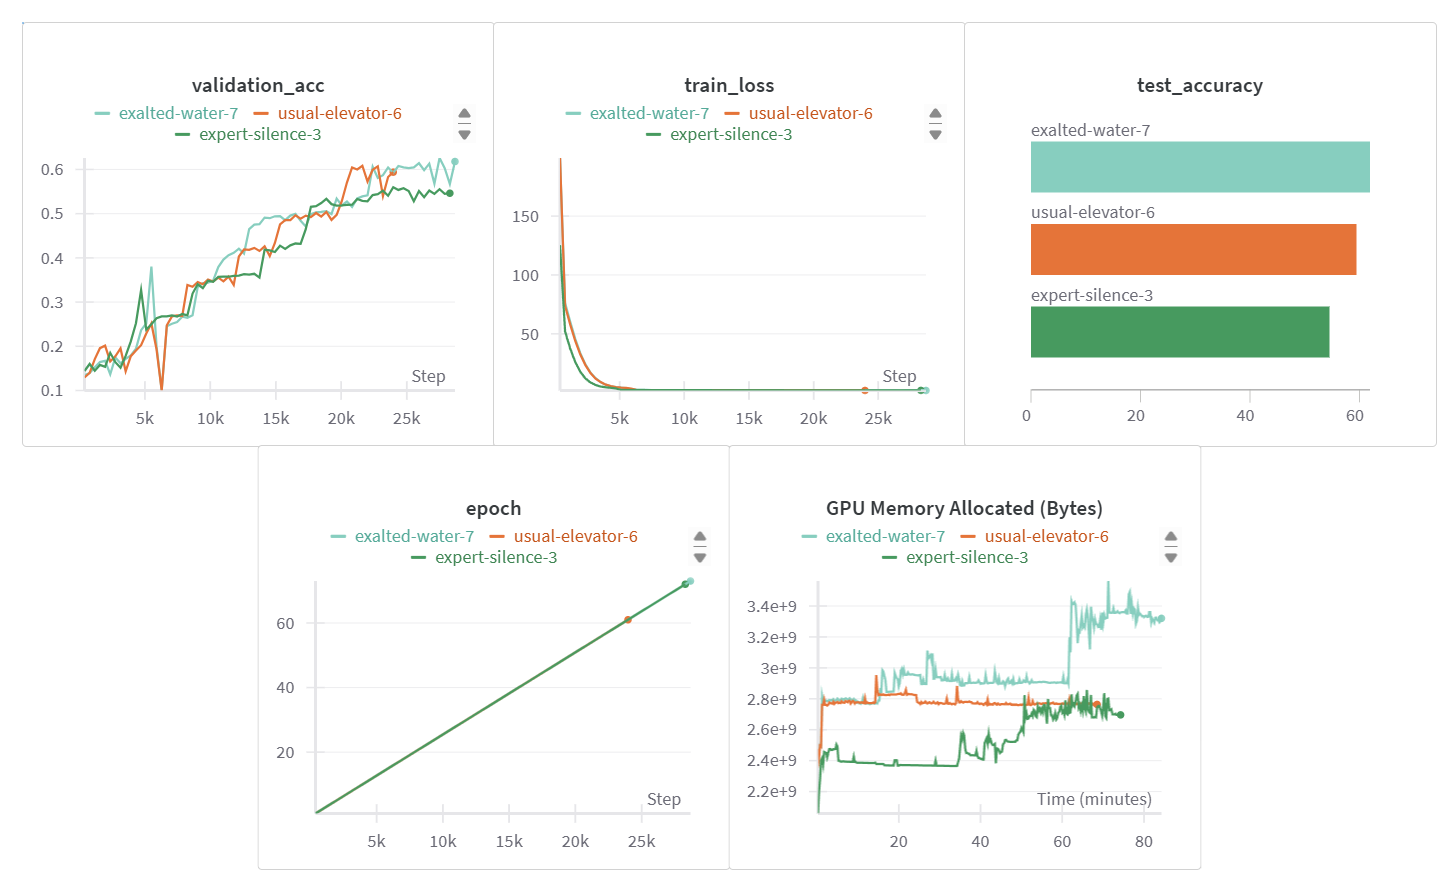
\includegraphics[width=6.26in,keepaspectratio]{images/NoProp-CT CIFAR-10.png}
    \caption{Графични резултати за NoProp-CT върху CIFAR-10}
\end{figure}

\begin{table}[H]
  \centering
  \renewcommand{\arraystretch}{1.5} % Увеличаване на вертикалния интервал
  \begin{tabular}{ccccc}
    \toprule
    \textbf{Име на изпълнение} & \textbf{Загуба} & \textbf{Тестова точност} & \textbf{Брой епохи} & \textbf{GPU памет (GB)}\\
    \midrule
    exalted-water-7& 1.8715& 61.79& 73& 3.17\\
    usual-elevator-6& 1.8880& 59.39& 61& 2.75\\
    expert-silence-3& 1.9260& 54.62& 72& 2.50\\
    \bottomrule
  \end{tabular}
  \caption{Метрики за различни изпълнения на NoProp-CT върху CIFAR-10}
  \label{tab:avg_metrics_noprop_ct_cifar-10}
\end{table}

\subsection{NoProp-CT и CIFAR-100}
\begin{figure}[H]
    \centering
    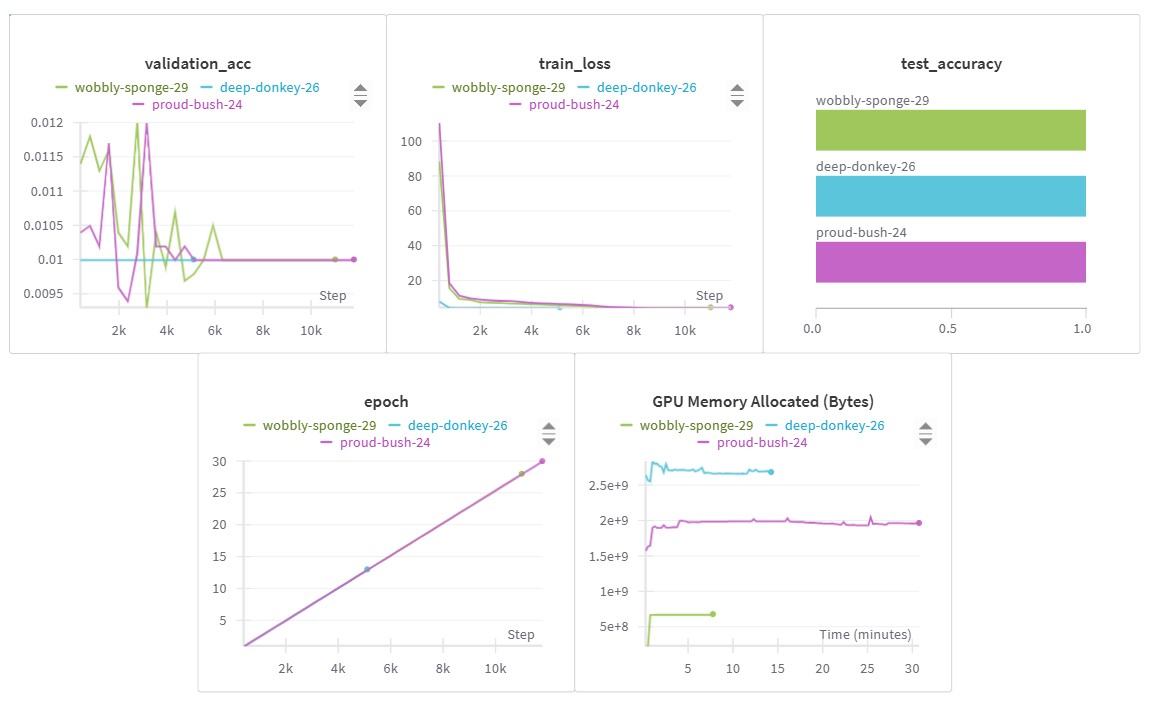
\includegraphics[width=6.26in,keepaspectratio]{images/NoProp-CT CIFAR100.jpg}
    \caption{Графични резултати за NoProp-CT върху CIFAR-100}
\end{figure}

\begin{table}[H]
  \centering
  \renewcommand{\arraystretch}{1.5} % Увеличаване на вертикалния интервал
  \begin{tabular}{ccccc}
    \toprule
    \textbf{Име на изпълнение} & \textbf{Загуба} & \textbf{Тестова точност} & \textbf{Брой епохи} & \textbf{GPU памет (GB)}\\
    \midrule
    wobbly-sponge-29 & 4.6167& 1 & 29 & 0.63 \\
    deep-donkey-26 & 4.6106 & 1 & 13 & 2.64 \\
    proud-bust-24 & 4.6209 & 1 & 30 & 1.91 \\
    \bottomrule
  \end{tabular}
  \caption{Метрики за различни изпълнения на NoProp-CT върху CIFAR-100}
  \label{tab:avg_metrics_noprop_ct_cifar-100}
\end{table}


\subsection{NoProp-CT и BLOODMNIST}
\begin{figure}[H]
    \centering
    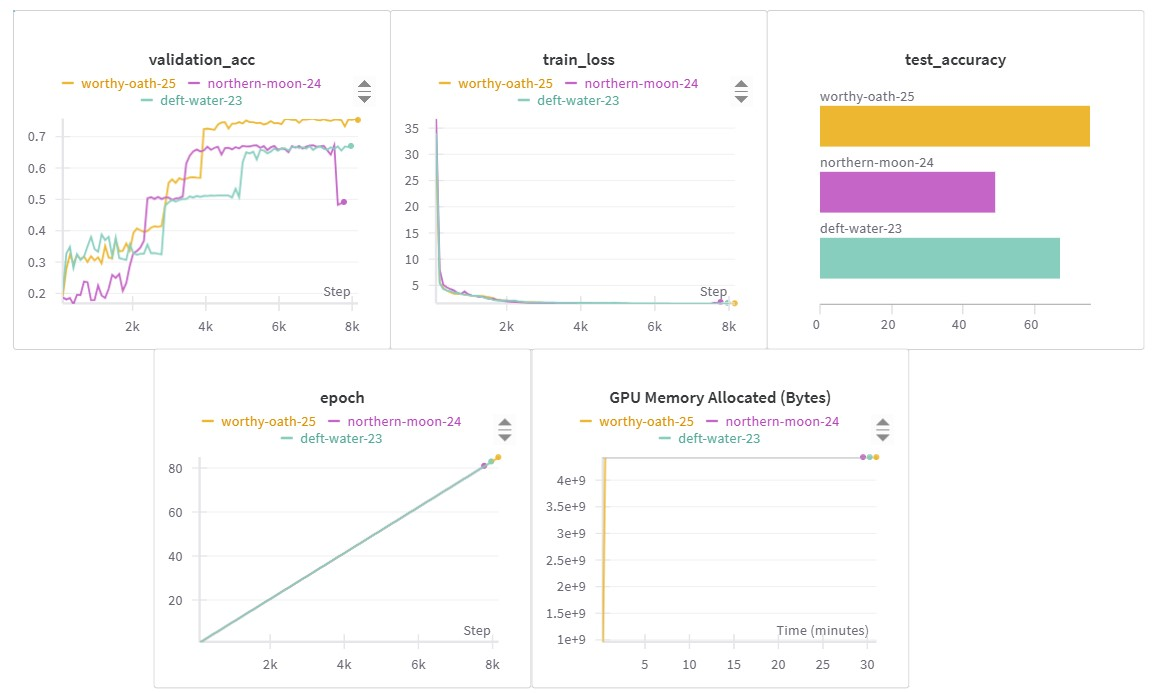
\includegraphics[width=6.26in,keepaspectratio]{images/NoProp CT BLOODMNIST.jpg}
    \caption{Графични резултати за NoProp-CT върху BLOODMNIST}
\end{figure}

\begin{table}[H]
  \centering
  \renewcommand{\arraystretch}{1.5} % Увеличаване на вертикалния интервал
  \begin{tabular}{ccccc}
    \toprule
    \textbf{Име на изпълнение} & \textbf{Загуба} & \textbf{Тестова точност} & \textbf{Брой епохи} & \textbf{GPU памет (GB)}\\
    \midrule
    worthy-oath-25 & 1.5700 & 75.50 & 85 & 4.43\\
    northern-moon-24 & 1.8103 & 49.08 & 81 & 4.43\\
    deft-water-23 & 1.6466 & 67.14 & 83 & 4.43\\
    \bottomrule
  \end{tabular}
  \caption{Метрики за различни изпълнения на NoProp-CT върху BLOODMNIST}
  \label{tab:avg_metrics_noprop_ct_bloodmnist}
\end{table}

\subsection{Сравнение с  оригиналните резултати}
\begin{table}[H]
    \centering
    % Requires \usepackage{booktabs, multirow}
    \begin{tabular}{llcccc}
    \toprule
    \multirow[b]{2}{*}{Dataset} & \multirow[b]{2}{*}{Split} & \multicolumn{2}{c}{NoProp-CT} & \multicolumn{2}{c}{NoProp-DT} \\
    \cmidrule(lr){3-4} \cmidrule(lr){5-6}
    & & Paper & Implementation & Paper & Implementation \\
    \midrule
    \multirow{2}{*}{MNIST}    & Train & $97.18\pm1.02$ &  $\mathbf{98.73\pm0.23}$& $\mathbf{99.97\pm0.0}$  &   $99.44\pm0.08$\\
                              & Test  & $97.17\pm0.94$&  $\mathbf{98.73\pm0.23}$& $\mathbf{99.54\pm0.04}$ &   $99.44\pm0.08$\\
    \midrule
    \multirow{2}{*}{CIFAR-10} & Train & $\mathbf{86.2\pm7.34}$  &  $58.6\pm3.65$& $\mathbf{97.23\pm0.11}$ &   $80.30\pm0.6$\\
                              & Test  & $\mathbf{66.54\pm3.63}$&  $58.6\pm3.65$& $\mathbf{80.54\pm0.2}$  &   $80.30\pm0.6$\\
    \midrule
    \multirow{2}{*}{CIFAR-100}& Train & $\mathbf{40.88\pm10.72}$ & $0.23$\dag & $\mathbf{90.7\pm0.14}$  &   $45.17\pm0.64$\\
                              & Test  & $21.31\pm4.17$&  $\mathbf{0.23}$\dag & $\mathbf{46.06\pm0.25}$&   $45.17\pm0.64$\\
    \midrule
    \multirow{2}{*}{MEDMNIST} & Train &               -&  $\mathbf{69.92\pm4.71}$&           -&   $\mathbf{98.39\pm0.24}$\\
                              & Test  &               -&  $\mathbf{63.90\pm13.50}$&                -&   $\mathbf{98.22\pm0.22}$\\
    \bottomrule
    \end{tabular}
    \caption{Сравнение на получените резултати от имплементацията с обявените резултати в оригиналната статия. \\
    \dag Тренирането на модела беше нестабилно}
    \label{table:results_transposed}
\end{table}

\subsection{Сравнение на използваната памет}
\begin{table}[H]
    \centering
    \begin{tabular}{lccc}
    \toprule
    \textbf{Вариант} & \textbf{MNIST} & \textbf{CIFAR-10} & \textbf{CIFAR-100} \\
    \midrule
    NoProp-DT & 1.54 GB & 1.15 GB & 0.89 GB \\
    \midrule
    NoProp-CT & 2.36 GB & 2.81 GB & 1.73 GB \\
    \bottomrule
    \end{tabular}
    \caption{Сравнение на употребата на GPU RAM памет на имплементацията за различни методи и набори от данни.}
    \label{table:memory_usage}
\end{table}

\newpage
\section{Заключение}

Проектът за имплементация и тестване на подхода за обучение \emph{NoProp} демонстрира съвпадение с цитираните в статията възможности на модела, което доказва коректността на имплементацията. Резултатите от тестовете върху разработката на екипа показват, че NoProp-DT постига висока точност на класификация върху наборите от данни MNIST (99.44 ± 0.08\%), CIFAR-10 (80.30 ± 0.6\%), CIFAR-100 (45.17 ± 0.64\%) и BLOODMNIST (98.22 ± 0.22\%), като в някои случаи надхвърля или се доближава до оригиналните резултати от статията. NoProp-CT, макар и с по-ниска производителност върху по-сложни набори като CIFAR-10 (58.6 ± 3.65\%) и CIFAR-100 (1\%), показва стабилност върху MNIST (98.73 ± 0.82\%).

Основните предимства на \emph{NoProp} включват възможността за паралелна обработка, намалени изисквания за памет и потенциал за ускоряване на обучението. Проект успешно имплементира \emph{NoProp-DT} и \emph{NoProp-CT}, като разширява тестването и върху набора \texttt{BLOODMNIST} от \texttt{MedMNIST+}. Резултатите демонстрират приложимостта на метода и към изображения с по-висока резолюция. 

За съжаление, екипът ни константира и някои (субективни) недостатъци на подхода, сред които:
\begin{itemize}
    \item значителна сложност на имплементацията в сравнение с \emph{backpropagation}
    \item повишена вероятност от бъгове и логически грешки, която наблюдавахме в други неофиционални имплементации\cite{githubPotentiallyIncorrect} и нашата собствена
    \item относителна нестабилност на тренирането, която не се наблюдава при \emph{backpropagation}
    \item голяма дисперсия и немонотонност в метриките на резултатите от тренирането. 
\end{itemize}

В заключение, екипът констатира, че NoProp е успешна алтернатива на съществуващите алгоритми без използване на \emph{backpropagation}, както и традиционните \emph{backpropagation} алгоритми в сценарии на паралелно обучение и ограниченa работна памет на хардуера. 
 
\bibliographystyle{plain}
\bibliography{references}

\end{document}
